\subsection{Grafos de Cayley}
Os grafos de Cayley são espaços métricos que podem ser naturalmente associados, a menos de quasi-isometria a um grupo finitamente gerado. Nesta seção apresentaremos a definição dos grafos de Cayley e algumas principais propriedades relacionadas.

Primeiro sejamos mais gerais, definamos grafos métricos.

\begin{definition}
Dado um grafo $\Gamma$ (um conjunto de vértices, identificados a pontos, e arestas, identificadas a caminhos) qualquer e uma função de comprimento (que atribuí um valor positivo para cada aresta), chamaremos \textbf{grafo métrico} correspondente a $\Gamma$ o espaço dado pela união dos vértices e de todos pontos das arestas com a métrica induzida pelo comprimento (ou o ínfimo dentre os caminhos possíveis).
\end{definition}

Discutamos agora os grafos de Cayley. Tomaremos $S$ um conjunto finito simétrico (tal que $S = \{ s^{-1} | \ s \in S \}$) e $G$ grupo gerado por $S$. Ou seja, $g \in G$ se e somente se $g$ pode ser escrito como combinação finita (dada a operação fixada para o grupo) de elementos de $S$.

\begin{definition}
Um \textbf{grafo de Cayley} $Cay(G, S)$ é um grafo métrico com conjunto de vértices $G$ e conjunto de arestas (todas com comprimento 1) em que liga-se $g,h \in G \iff \exists s \in S$ tal que $h=gs$.
\end{definition}

É interessante verificar que grafos de Cayley são espaços métricos próprios (no sentido em que toda bola fechada é compacta) e geodésicos (no sentido da definição \ref{esp_geo}).

Note que, por construção, toda aresta é compacta. Daí, toda bola fechada, por conter finitas arestas (decorre-se de $S$ finito, pois há no máximo $|S|$ arestas saindo do cada vértice), é compacta.

Pela construção de grafo métrico, há uma geodésica entre quaisquer dois pontos conexos. Como $S$ gera $G$, segue que $Cay(G,S)$ é fortemente conexo e, por isso, geodésico.

Para visualizar exemplos de grafos de Cayley, observemos novamente os espaços da figura \ref{figure:cay(Z)} e notemos que se tratam de, respectivamente, $Cay(\mathbb{Z}, \{ \pm 1 \})$ e $Cay(\mathbb{Z}, \{ \pm 2, \pm 3 \})$.

Outro exemplo, bem parecido com os anteriores, é $Cay(\mathbb{Z}^2, \{\pm(0, 1), \pm(0, 1) \})$. Que está desenhado na figura \ref{figure:cay(Z2)}.

\begin{figure}[ht]
  \centering
  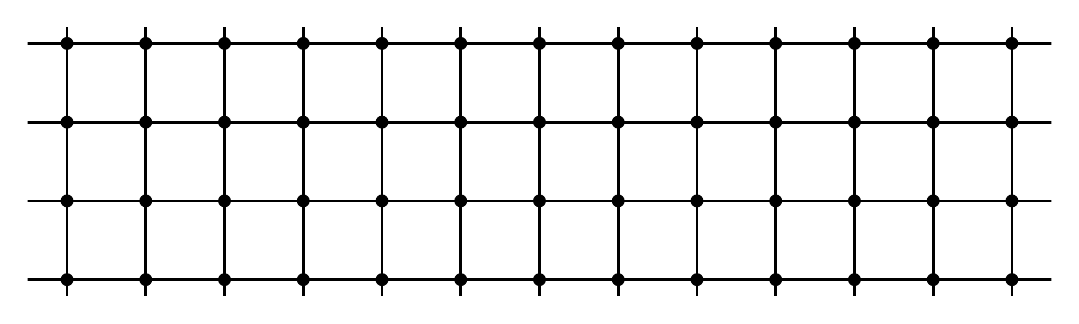
\begin{tikzpicture}
    \coordinate (Origin)   at (0,0);
    \coordinate (XAxisMin) at (-3,0);
    \coordinate (XAxisMax) at (5,0);
    \coordinate (YAxisMin) at (0,-2);
    \coordinate (YAxisMax) at (0,5);
    \begin{scope}
    \clip (-6.5,-0.2) rectangle (6.5,3.2);

    \foreach \x in {-6,-5,...,6}{% Two indices running over each
      \foreach \y in {0,1,...,6}{% node on the grid we have drawn 
        \draw[line width=1pt](\x-1,\y)--(\x+1,\y);
        \draw[line width=1pt](\x,\y-1)--(\x,\y+1);
        \node[draw,circle,inner sep=1.5pt,fill] at (\x,\y) {};
            % Places a dot at those points
      }
    }
    \end{scope} 
  \end{tikzpicture}
  \caption{O espaço $Cay(\mathbb{Z}^2, \{\pm(0, 1), \pm(0, 1) \})$.}
  \label{figure:cay(Z2)}
\end{figure}

Um último exemplo, para um grupo finito, está na figura \ref{figure:cayfin}, onde nota-se que podemos identificar $Cay(\mathbb{Z}/n, \{\pm1 \})$ a um polígono de $n$ lados.

\begin{figure}[ht]
  \centering
  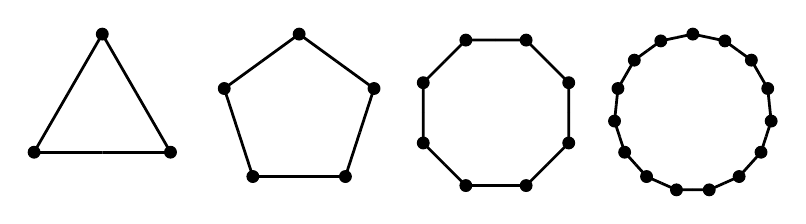
\begin{tikzpicture}
  \newcommand\polygon[2][]{
  \pgfmathsetmacro{\angle}{360/#2}
  \pgfmathsetmacro{\startangle}{-90 + \angle/2}
  \pgfmathsetmacro{\y}{cos(\angle/2)}
  \begin{scope}[#1]
    \foreach \i in {1,2,...,#2} {
      \pgfmathsetmacro{\x}{\startangle + \angle*\i}
      \draw[line width=1pt] (\x:1 cm) -- (\x + \angle/2:\y cm) -- cycle;
      \draw[line width=1pt] (\x + \angle/2:\y cm) -- (\x + \angle:1 cm) -- cycle;
      \node[draw,circle,inner sep=1.5pt,fill] at (\x + \angle:1 cm) {};
    }
  \end{scope}}
    \begin{scope}
    %\clip (-6.5,-0.2) rectangle (6.5,3.2);
    \polygon{3}
    \polygon[xshift=2.5cm]{5}
    \polygon[xshift=5cm]{8}
    \polygon[xshift=7.5cm]{15}
    \end{scope} 
  \end{tikzpicture}
  \caption{Os espaços $Cay(\mathbb{Z}/n, \{\pm1 \})$ para $n$ respectivamente igual a 3, 5, 8 e 15.}
  \label{figure:cayfin}
\end{figure}

Agora, como queremos estudar um grupo independentemente de seu conjunto gerador, é interessante notar que a escolha de $S$ "nunca interfere demais" na natureza de $Cay(G,S)$. Essa característica procede do seguinte lema.

\begin{lemma}
$Cay(G,S)$ é único a menos de quasi-isometria. Ou seja, para dois geradores finitos $S$ e $S'$ de $G$, há uma quasi-isometria natural $Cay(G,S) \rightarrow Cay(G,S')$.

\textbf{Prova:} Assumamos $G$ gerado pelos conjuntos finitos simétricos $S$ e $S'$. Seja $\Psi: Cay(G,S) \rightarrow Cay(G,S)$ tal que identifique todo elemento do espaço ao vértice mais próximo. Note que $\Psi$ é (1, 1)-quasi-isometria.

Seja $\Psi': Cay(G,S') \rightarrow Cay(G,S')$ da mesma forma que $\Psi$. Trivialmente, a inclusão da imagem de $\Psi$ em $Cay(G,S')$ também é (1, 1)-quasi-isometria.

Assim, como a composição de quasi-isometrias é quasi-isometria (não provamos esse fato aqui, mas segue diretamente da definição), para que tenhamos a proposição do lema verdadeira é apenas necessário que tracemos uma quasi-isometria entre as imagens de $\Psi$ e $\Psi'$.

Note que os elementos de ambas as imagens são os mesmos de $G$ e o que difere os espaços em questão é a métrica herdada da escolha do conjunto gerador. Chamaremos as distâncias de interesse $d_S$ e $d_{S'}$ e provaremos que a identidade $G \rightarrow G$ é quasi-isometria.

Agora, sendo $1 \in G$ o elemento neutro do grupo, da definição de grafo de Cayley, há aresta entre $g, h \in G$ se e somente se $\exists s \in S$ tal que $h=gs \Rightarrow g^{-1}h = s$. Daí, segue $d_S(g, h) = d_S(g^{-1}h, 1)$. Também notemos que $d_S(g, 1) = N \iff \exists$ um menor conjunto $\{s_1, ..., s_N\} \subset S$ tal que $g = s_1 ... s_N$.

Mostraremos que a distorção entre as métricas é limitada à proporcional a uma constante. Primeiro definiremos essa constante, "o numero máximo de elementos de um grupo que é necessário para reescrever um elemento do outro", como $M = max\{d_{S'}(s,1), d_{S}(s',1) : s \in S, s' \in S'\}$.

Enfim, assumamos, para quaisquer elementos de $G$, $d_{S}(g, h) = k$. Daí, existe $\{s_1, ..., s_k\} \subset S$ tal que $g^{-1}h = s_1 ... s_k$. De ser $S'$ gerador e, como $S \subset G$, temos $s_i = s'_{i,1} ... s'_{i,M_i}$ para todo $i \in \{1, ..., k\}$.

Portanto, $g^{-1}h = (s'_{1,1} ... s'_{1,M_1}) ... (s'_{k,1} ... s'_{k,M_k})$ e, como $\forall M_i$, $M_i \leq M$, temos
\[
d_{S'}(g, h) = d_{S'}(g^{-1}h, 1) \leq Mk = M d_{S}(g, h).
\]

A identidade é obviamente sobrejetiva e, com o mesmo argumento descrito, é possível provar (ao aplicá-lo "ao contrário", para o outro lado da desigualdade, $d_{S}(g, h) \leq M d_{S'}(g, h)$) que é mergulho quasi-isométrico. Assim, a identidade é quasi-isométrica e satisfaz-se a proposição. \qed
\end{lemma}

%\subsubsection{Ações de um Grupo}